\documentclass[12pt,a4paper]{article}

\usepackage[utf8]{inputenc}
\usepackage[T1]{fontenc}
\usepackage[magyar]{babel}
\usepackage{geometry}
\usepackage{graphicx}
\usepackage{float}
\usepackage{caption}
\usepackage{siunitx}

\geometry{margin=2.5cm}
\sisetup{locale = DE}
\renewcommand{\figurename}{Kép}

\begin{document}

\begin{titlepage}
    \centering
    \vspace*{3cm}

    {\Large \textbf{NÁR jegyzőkönyv}}\\[1cm]
    {\huge \textbf{Képes dokumentáció}}\\[2cm]

    \begin{tabular}{rl}
        Tárgy: & \textbf{NÁR} \\
        Készítette: & \textbf{Csirke Dániel} \\
        Dátum: & \textbf{\today} \\
    \end{tabular}

    \vfill
\end{titlepage}

\section{Képes dokumentáció}

\begin{figure}[H]
    \centering
    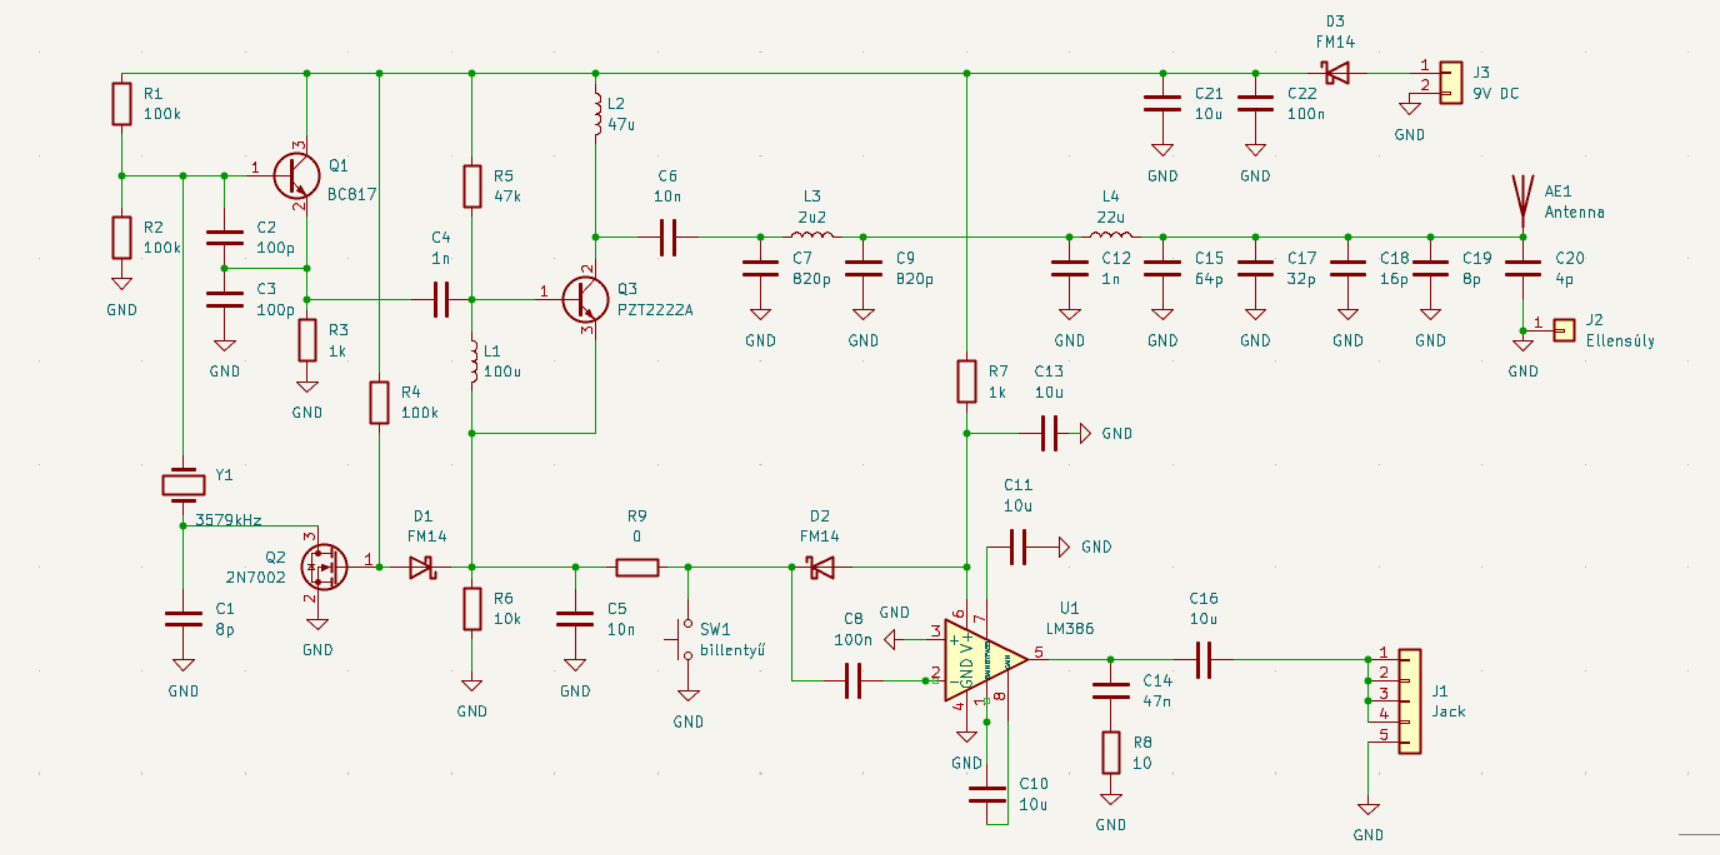
\includegraphics[width=\textwidth]{1sch.png}
    \caption{Kapcsolási rajz}
\end{figure}

\begin{figure}[H]
    \centering
    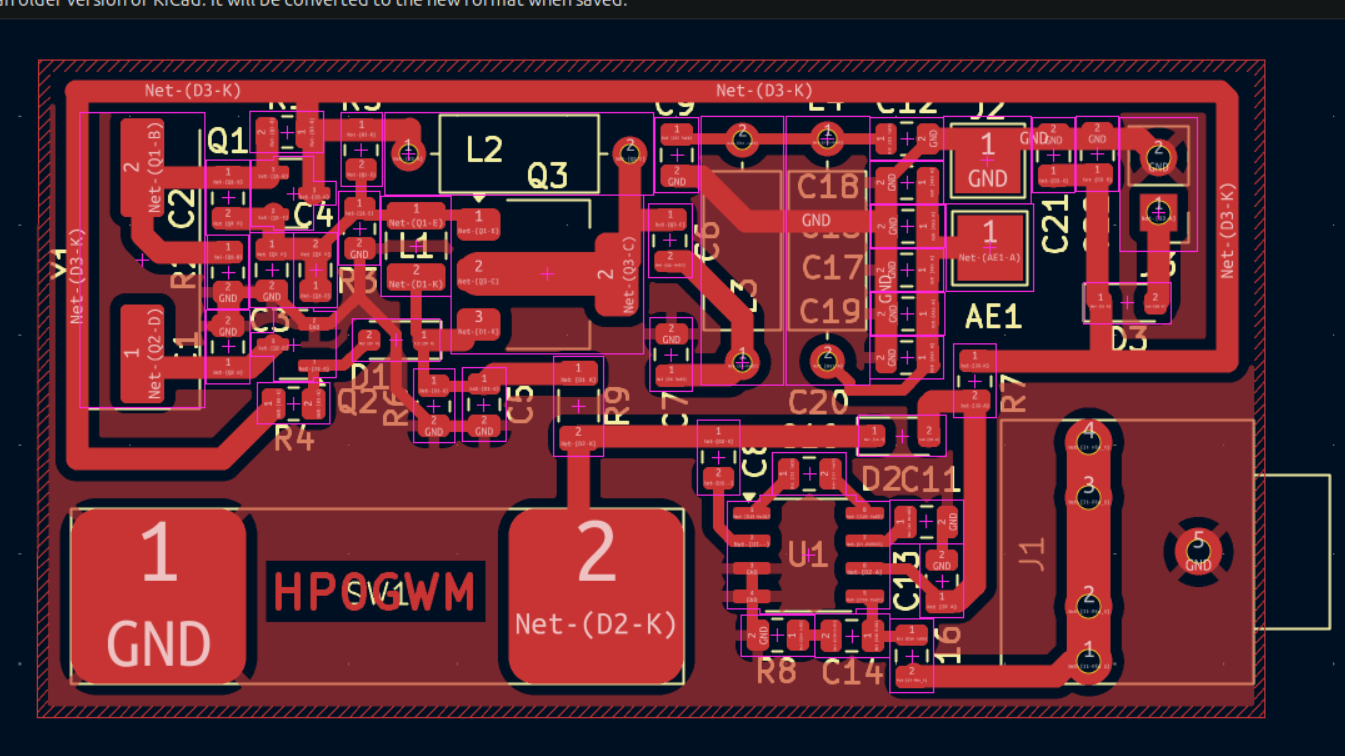
\includegraphics[width=\textwidth]{2layout.png}
    \caption{Rajzolat}
\end{figure}

\begin{figure}[H]
    \centering
    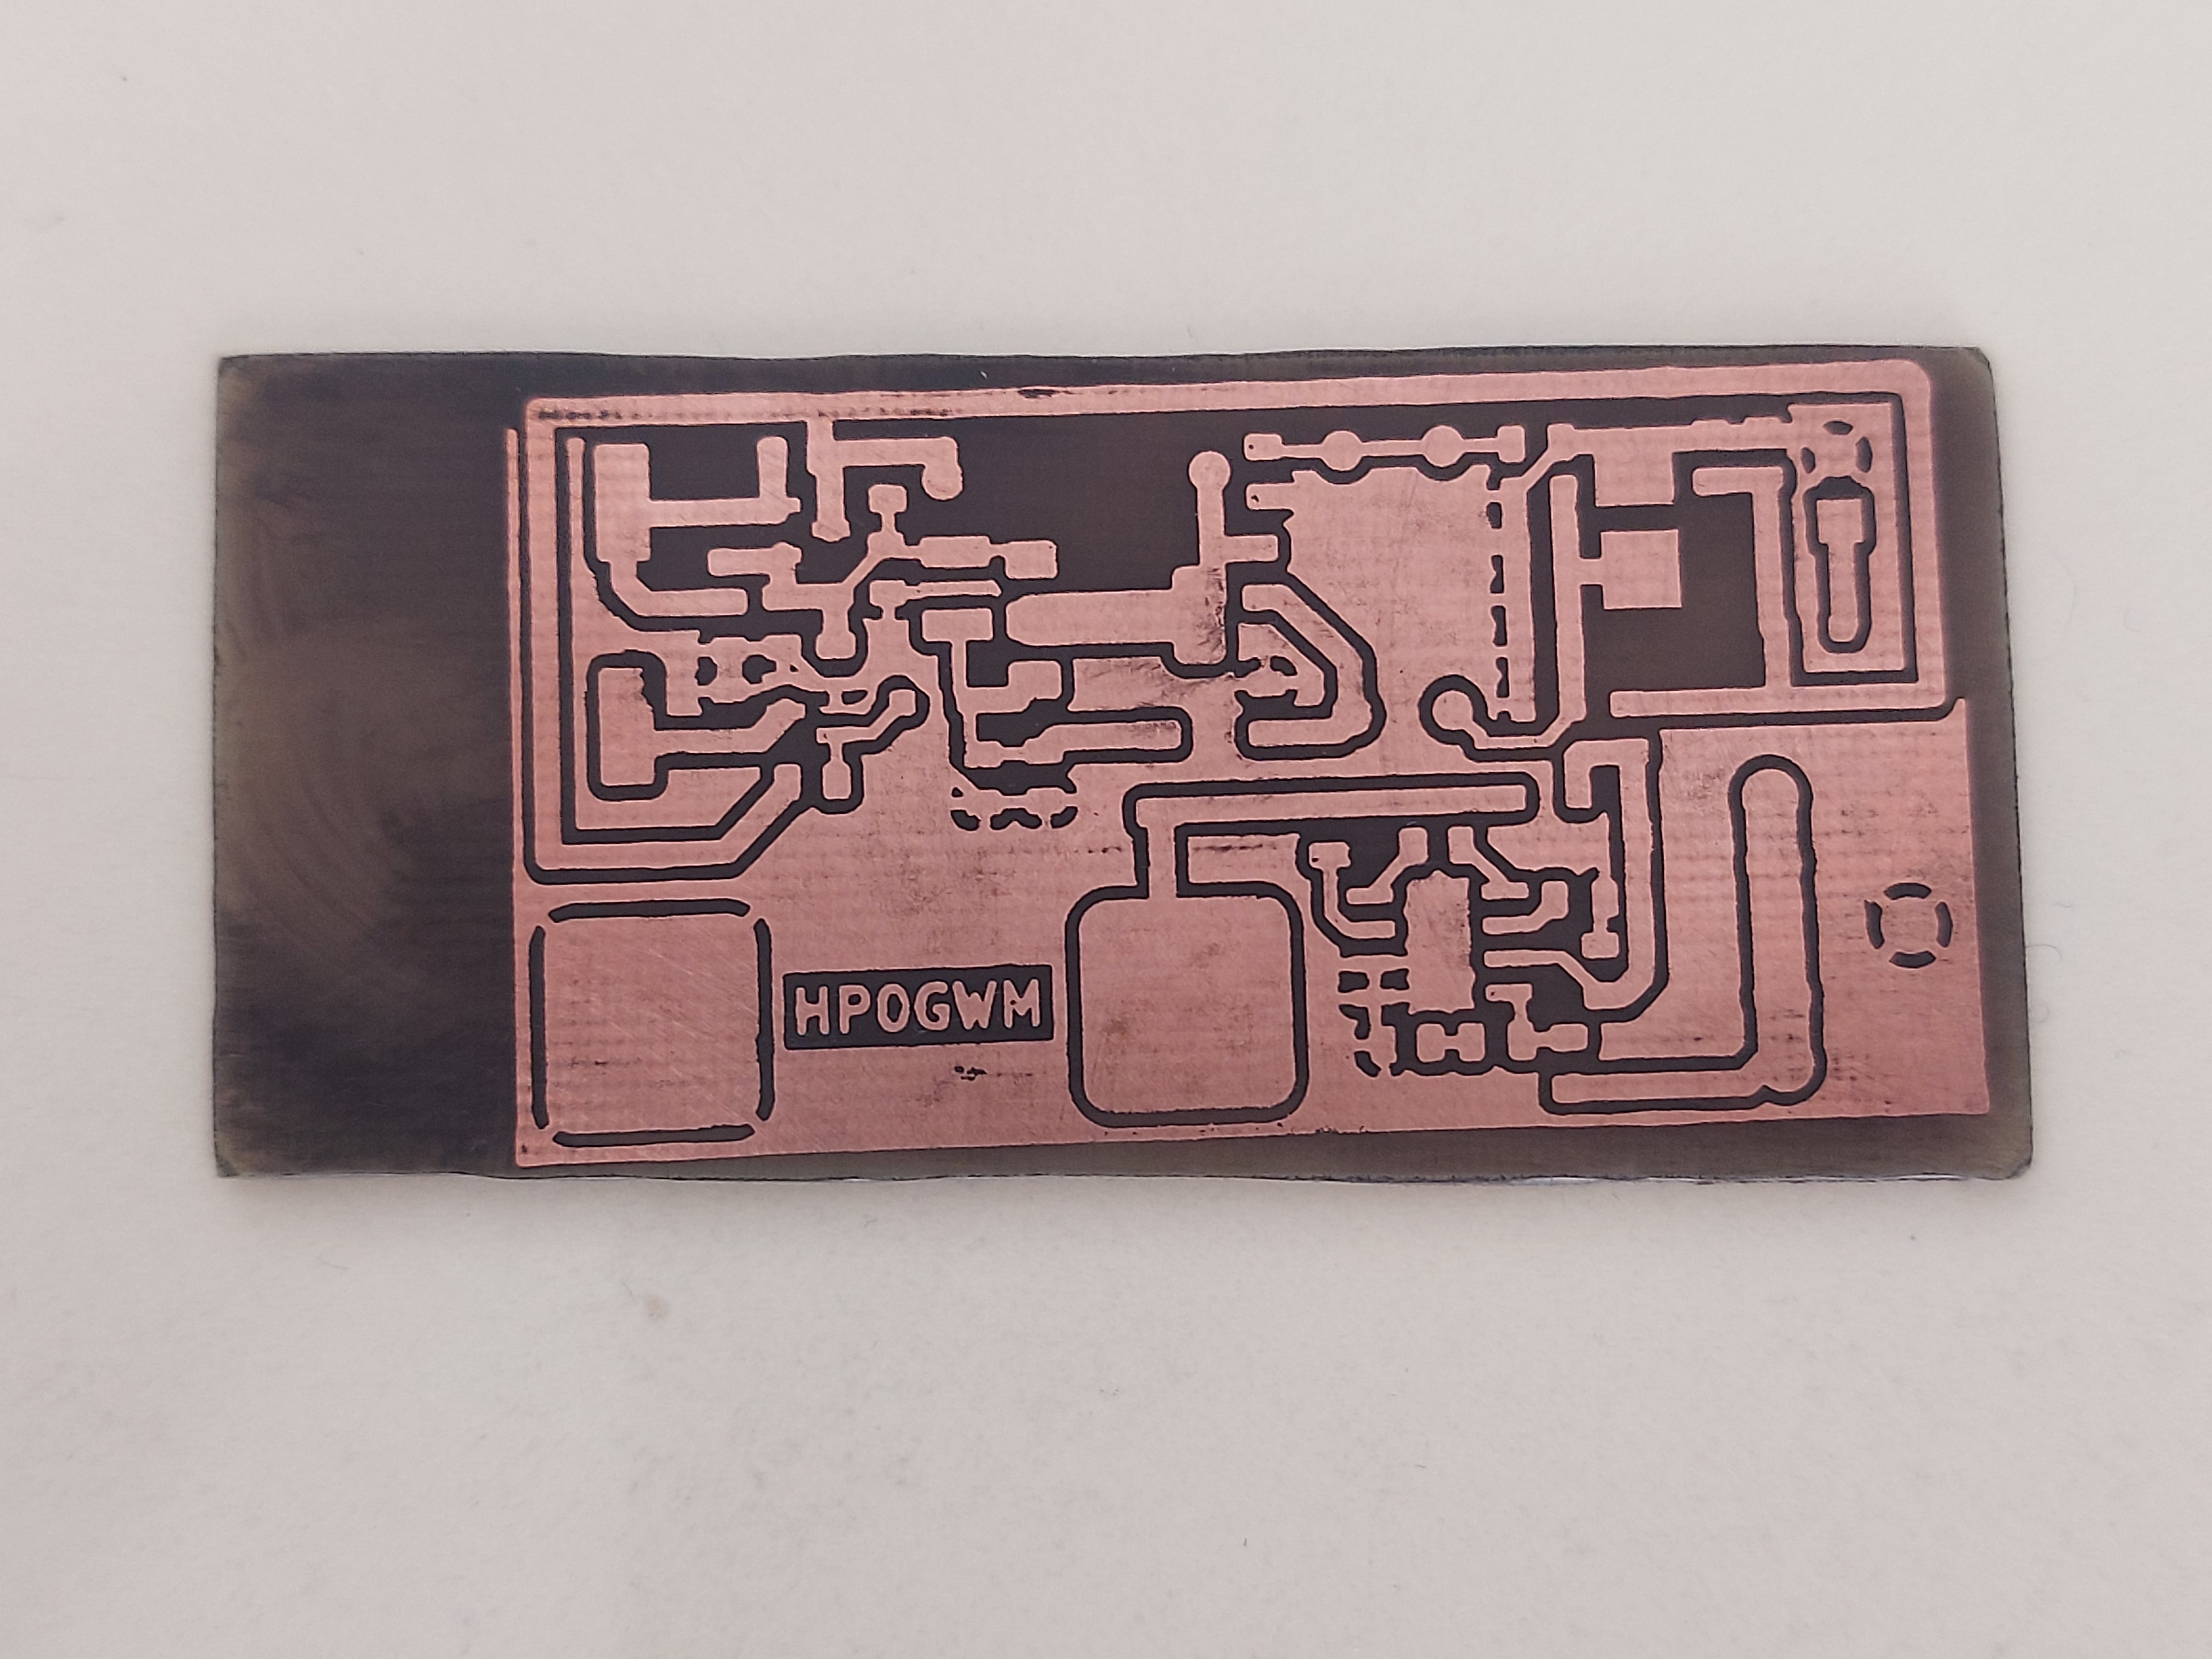
\includegraphics[width=\textwidth]{3etched.jpg}
    \caption{A lemart nyák}
\end{figure}

\begin{figure}[H]
    \centering
    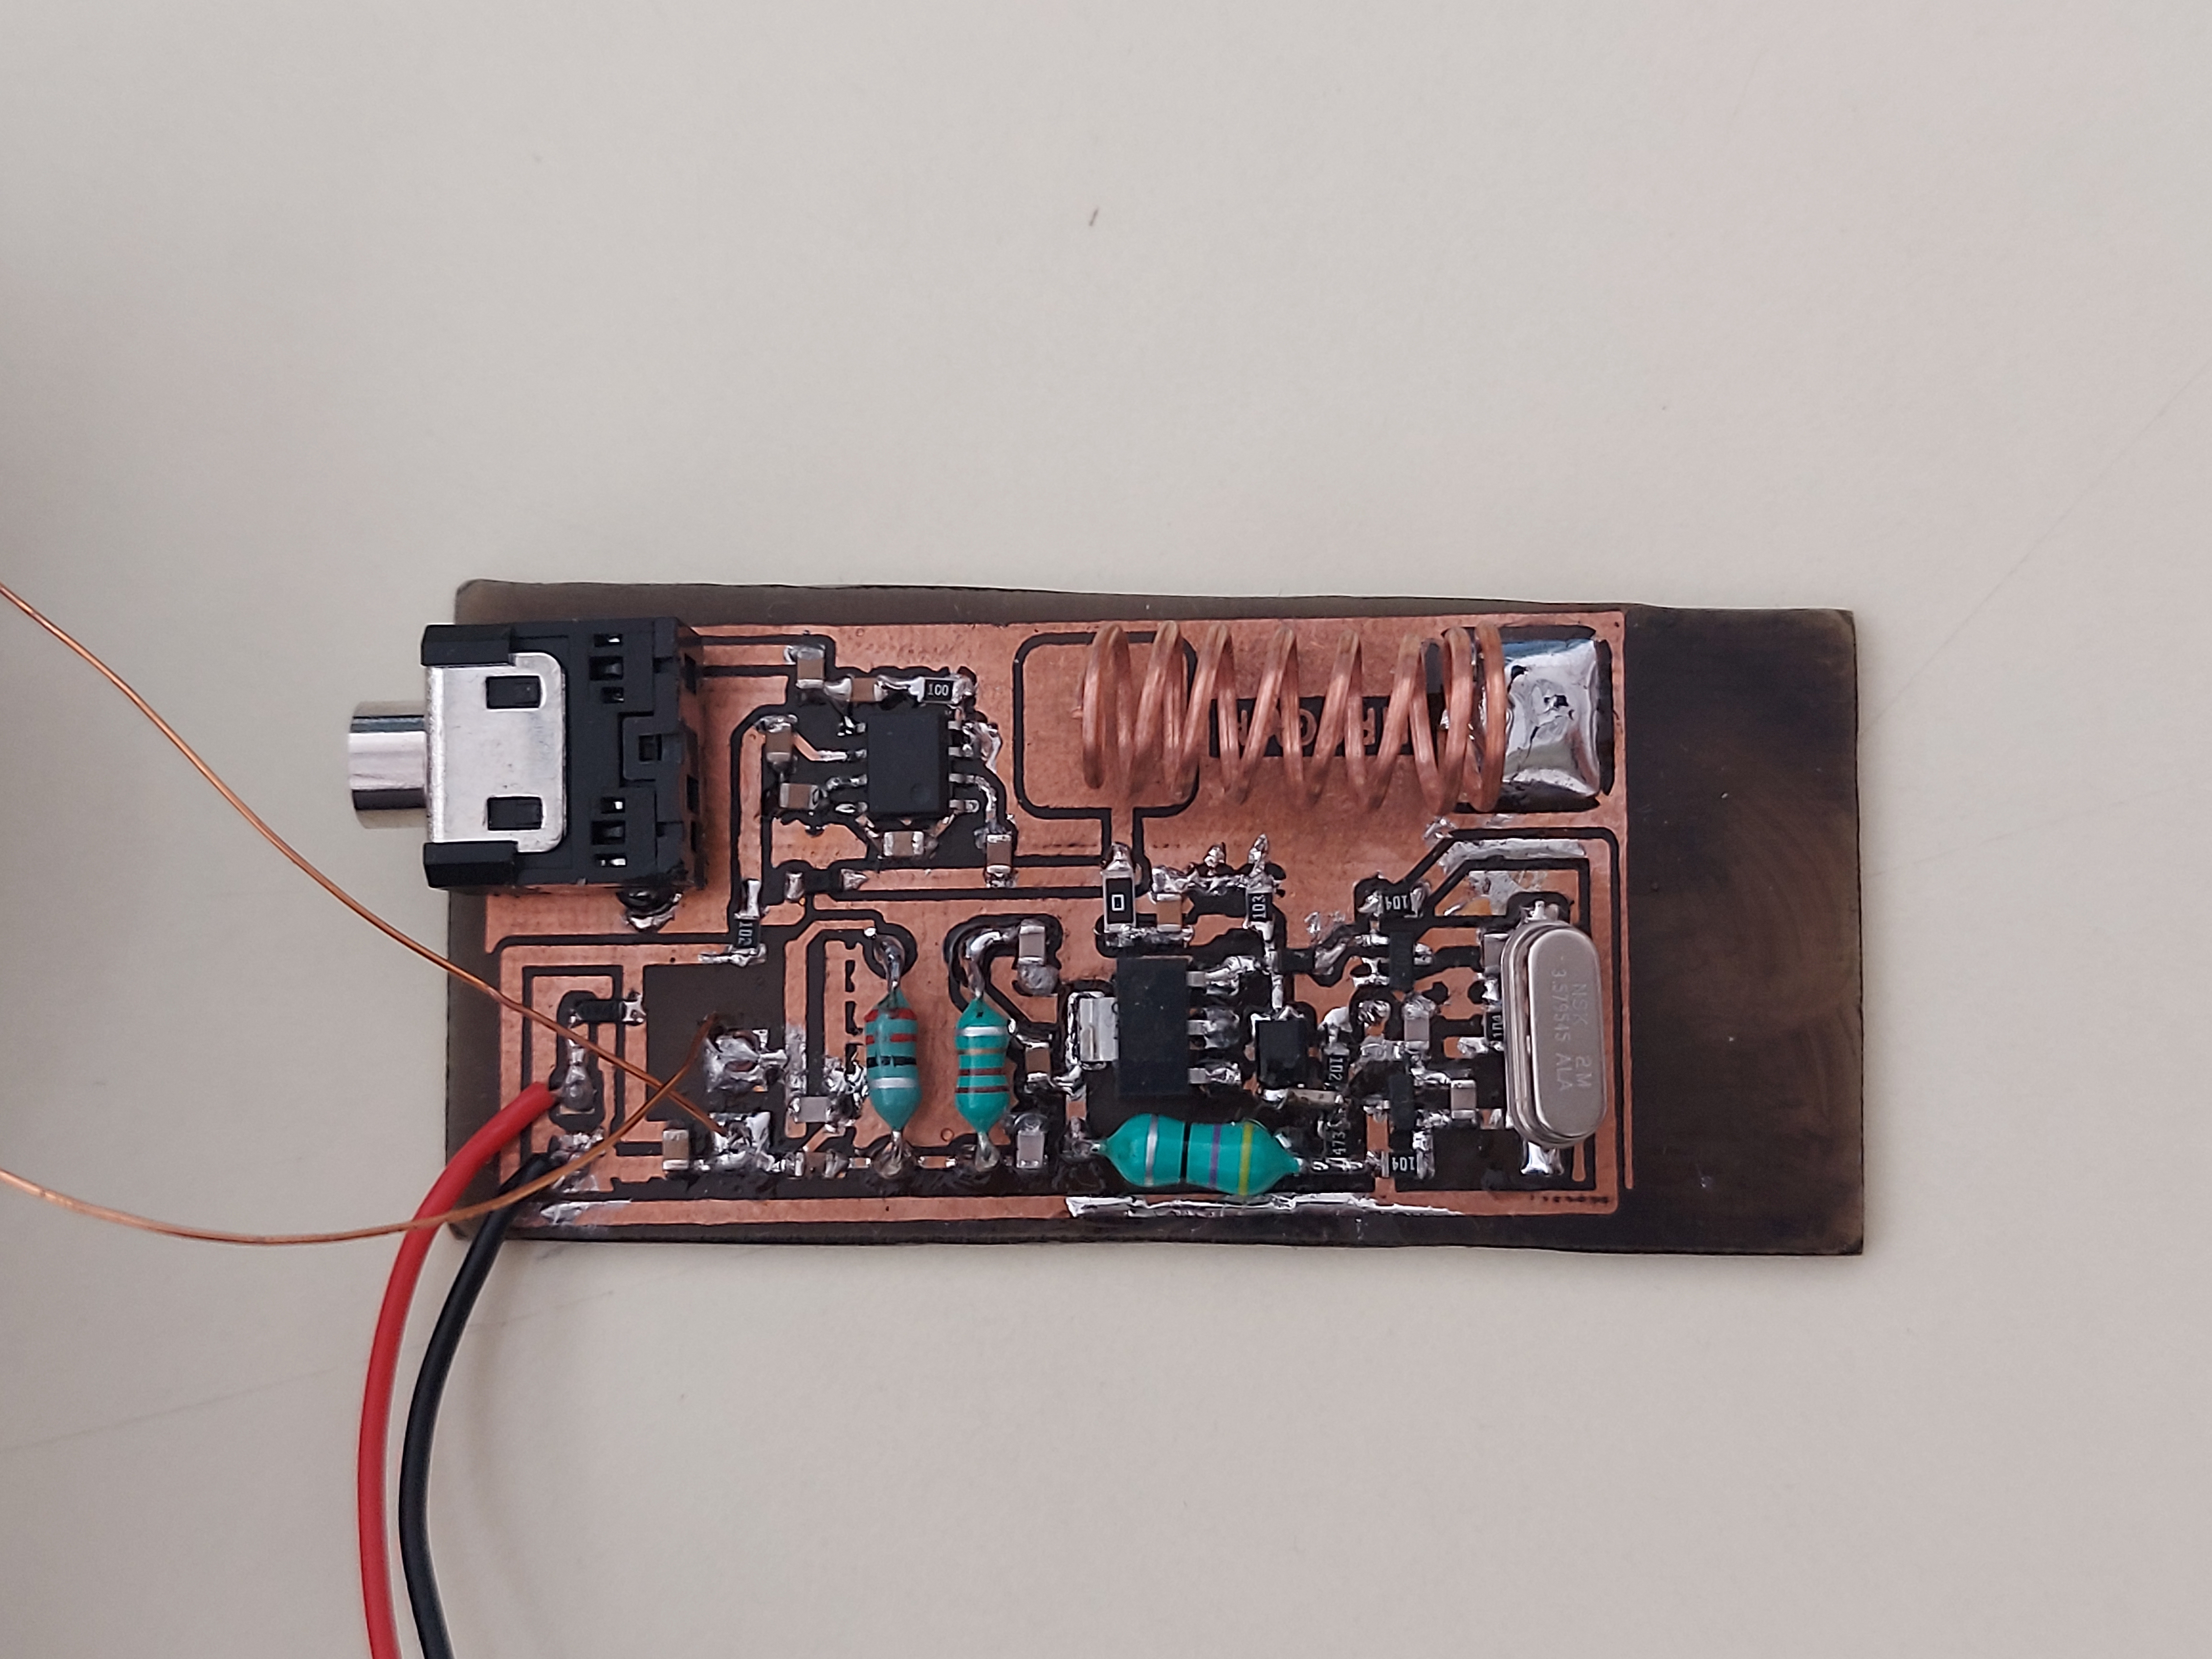
\includegraphics[width=0.8\textwidth]{4placed.jpg}
    \caption{A beültetett nyák}
\end{figure}

\begin{figure}[H]
    \centering
    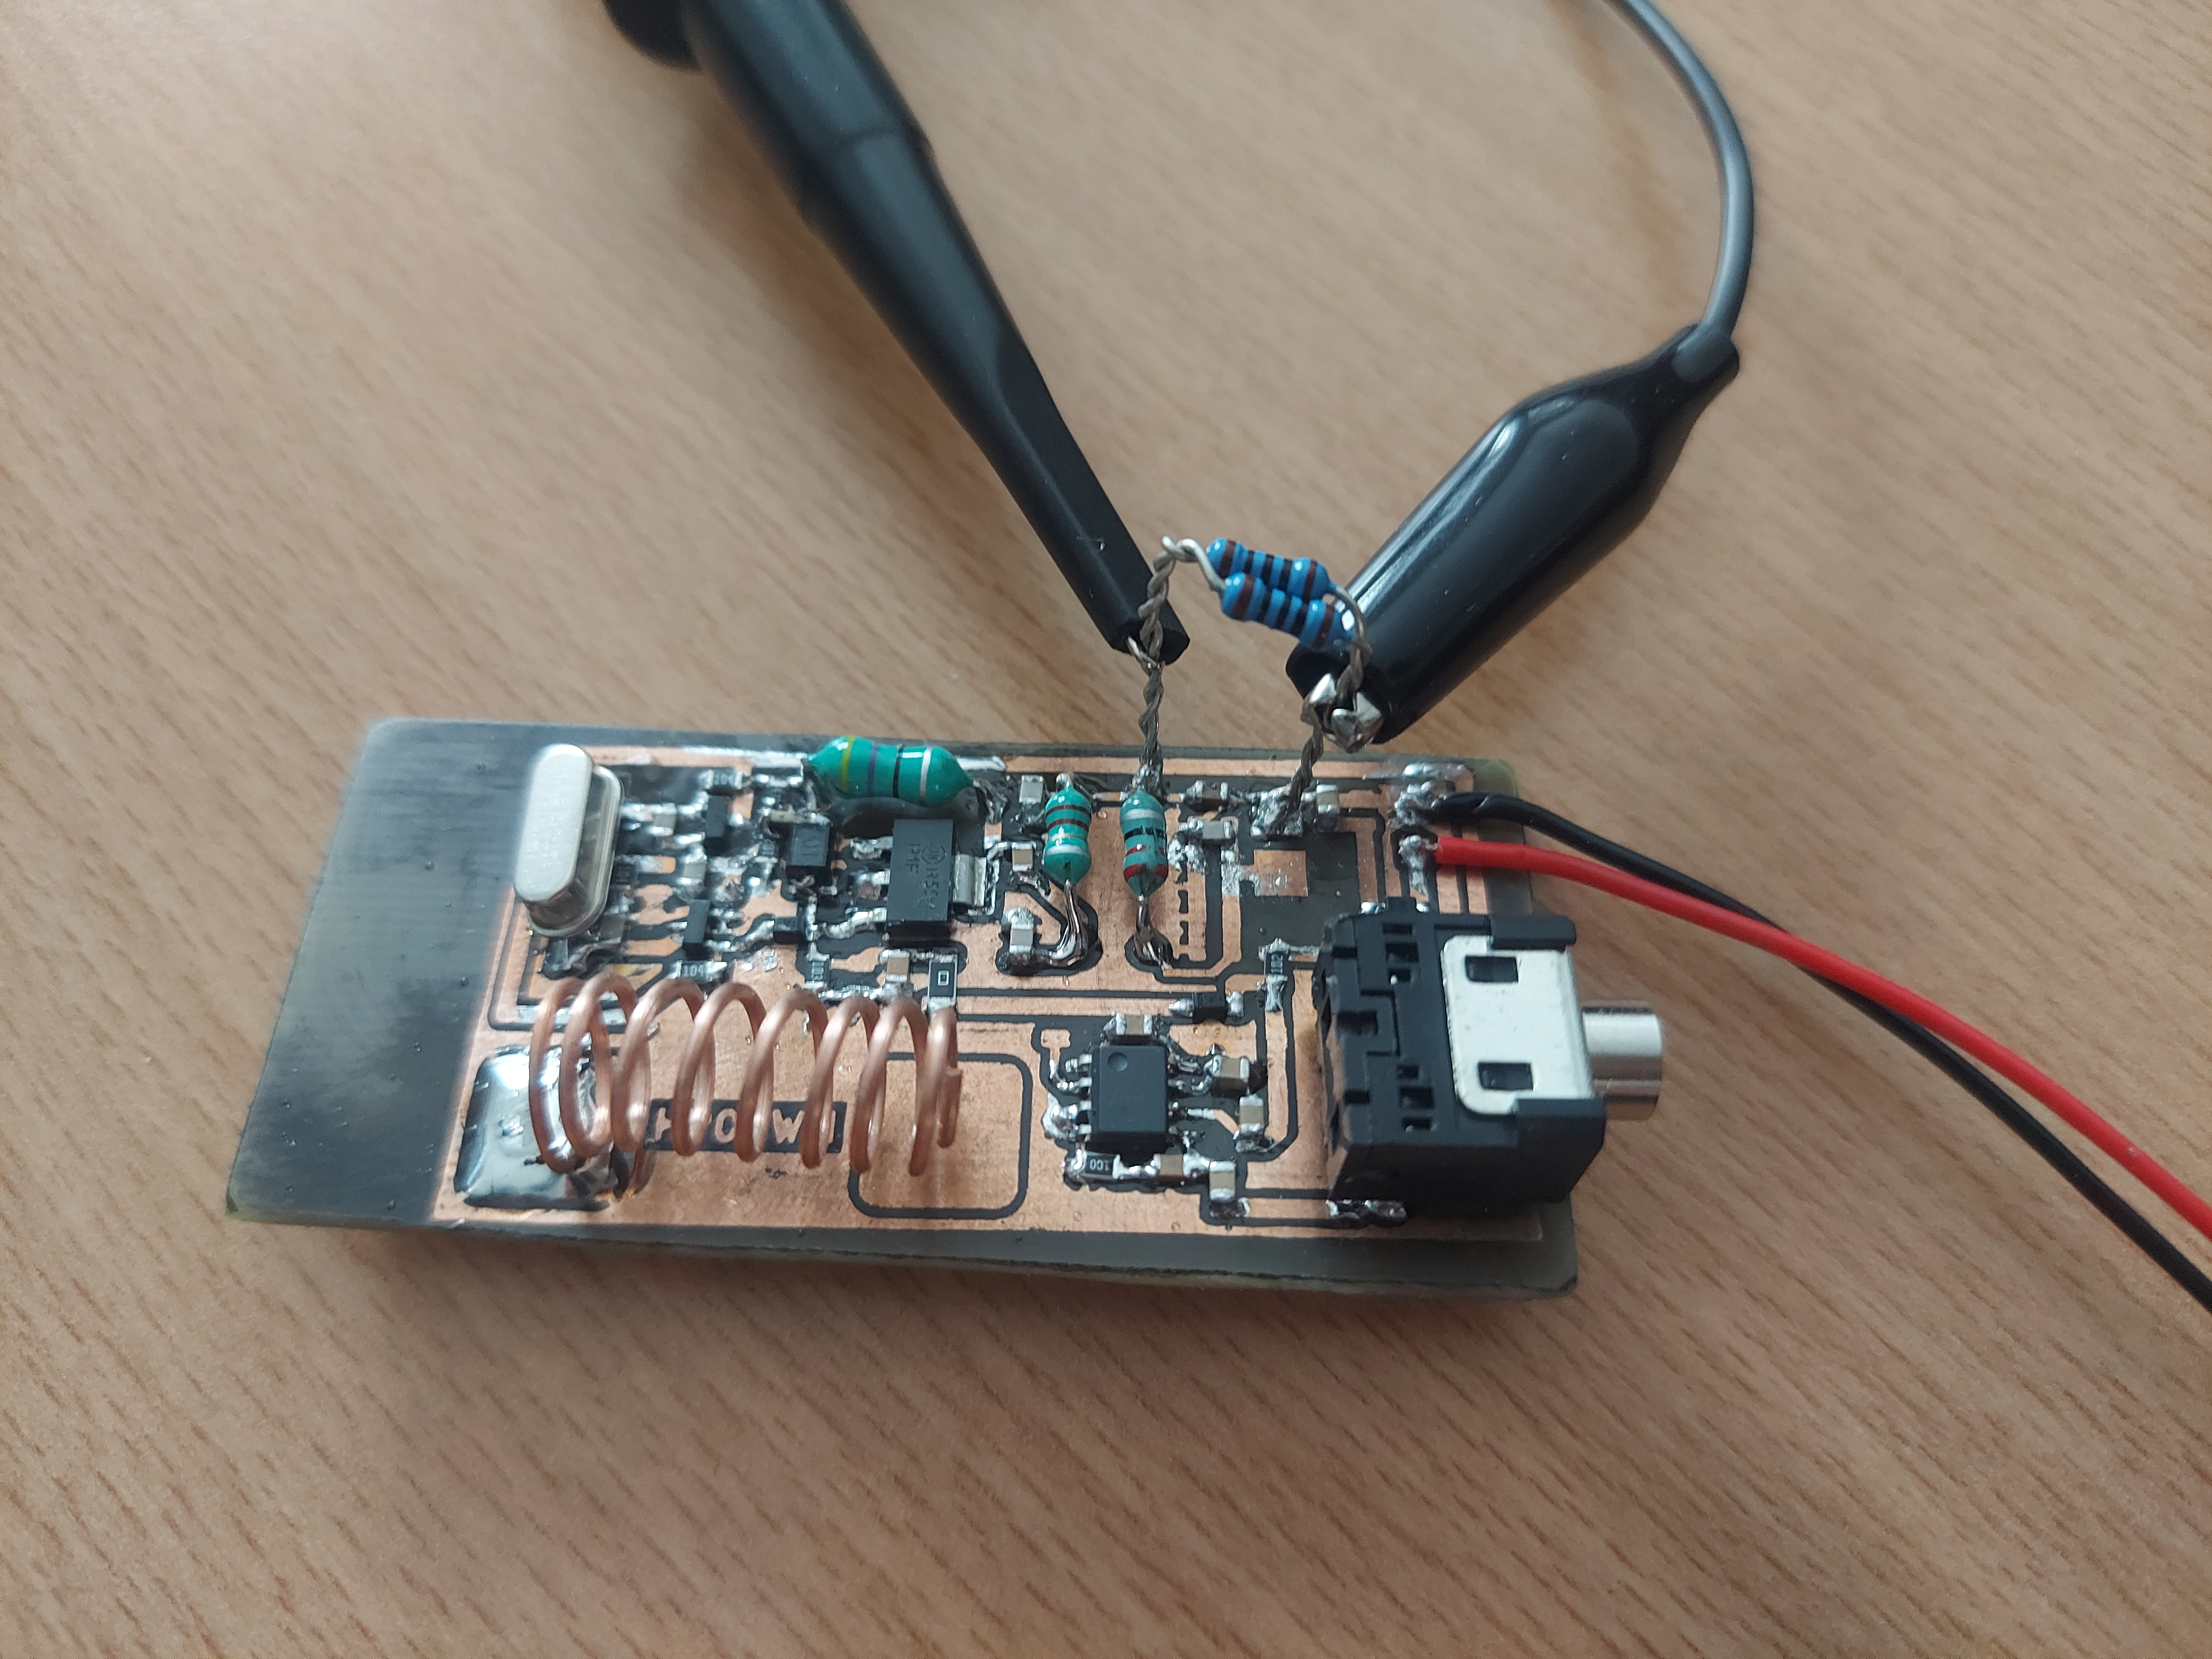
\includegraphics[width=\textwidth]{5measure.jpg}
    \caption{Mérési összeállítás \SI{50}{\ohm} műterhen}
\end{figure}

\begin{figure}[H]
    \centering
    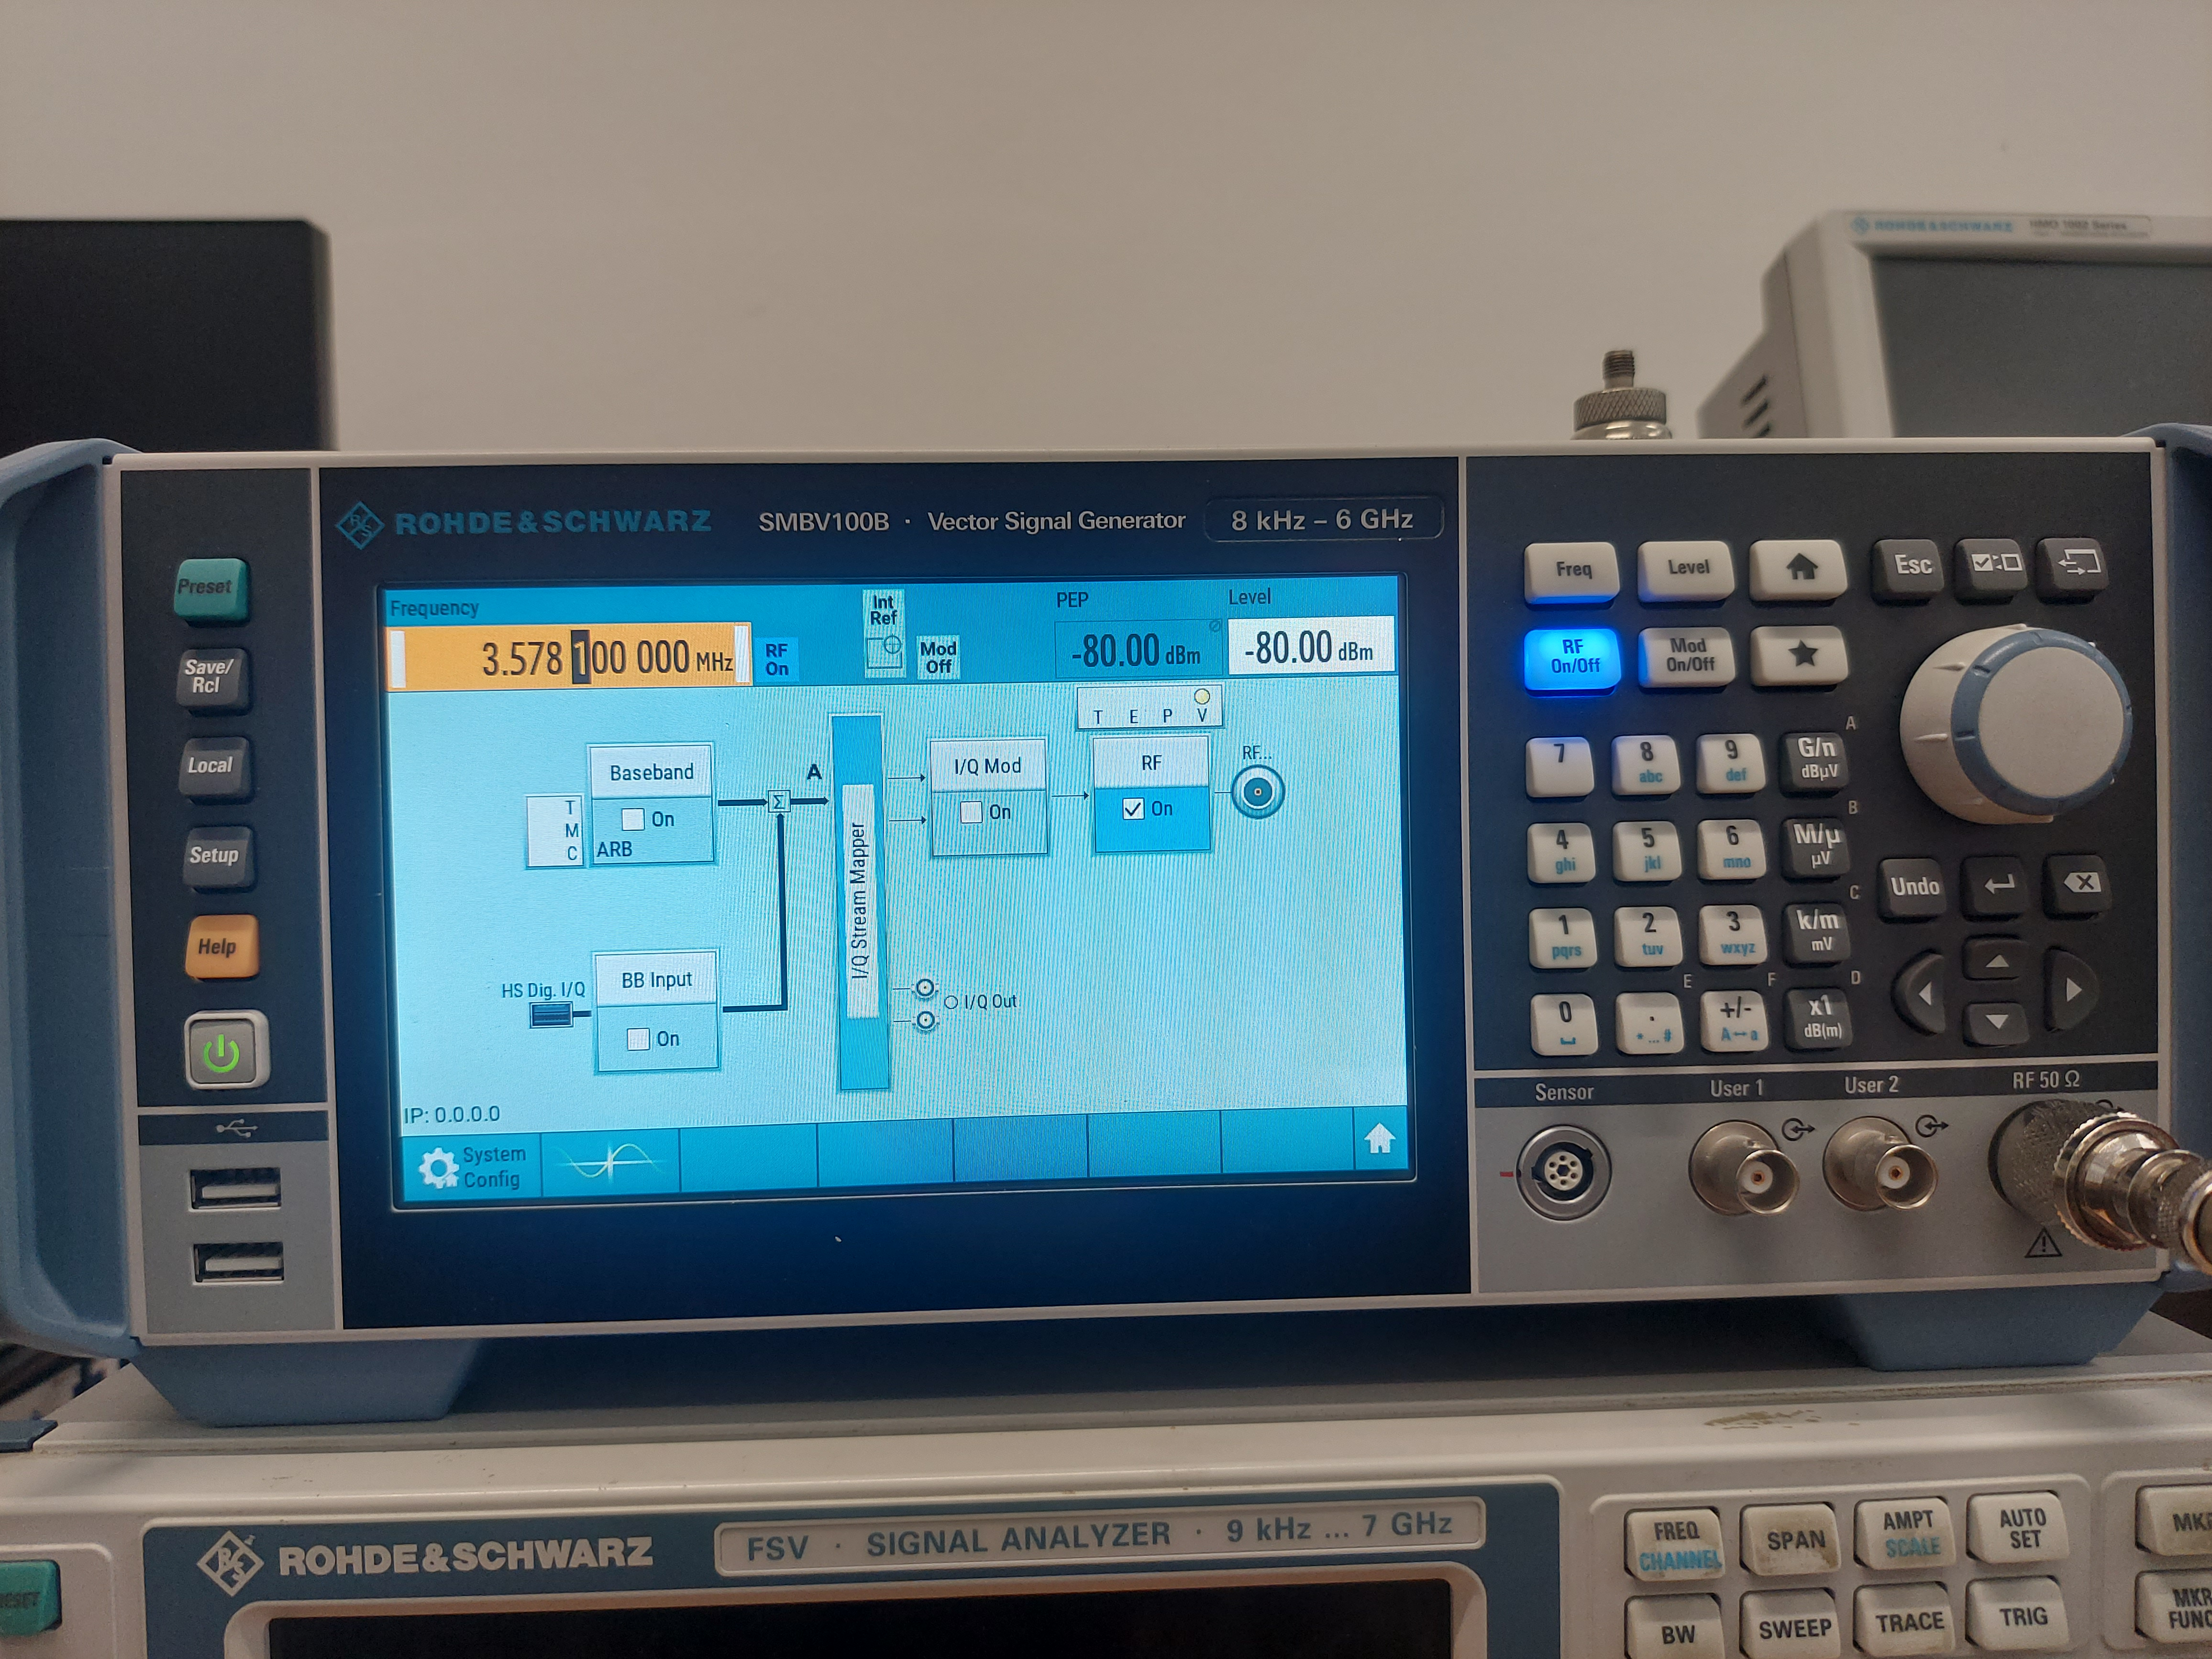
\includegraphics[width=\textwidth]{6measure_rx.jpg}
    \caption{Vétel mérése}
\end{figure}

\begin{figure}[H]
    \centering
    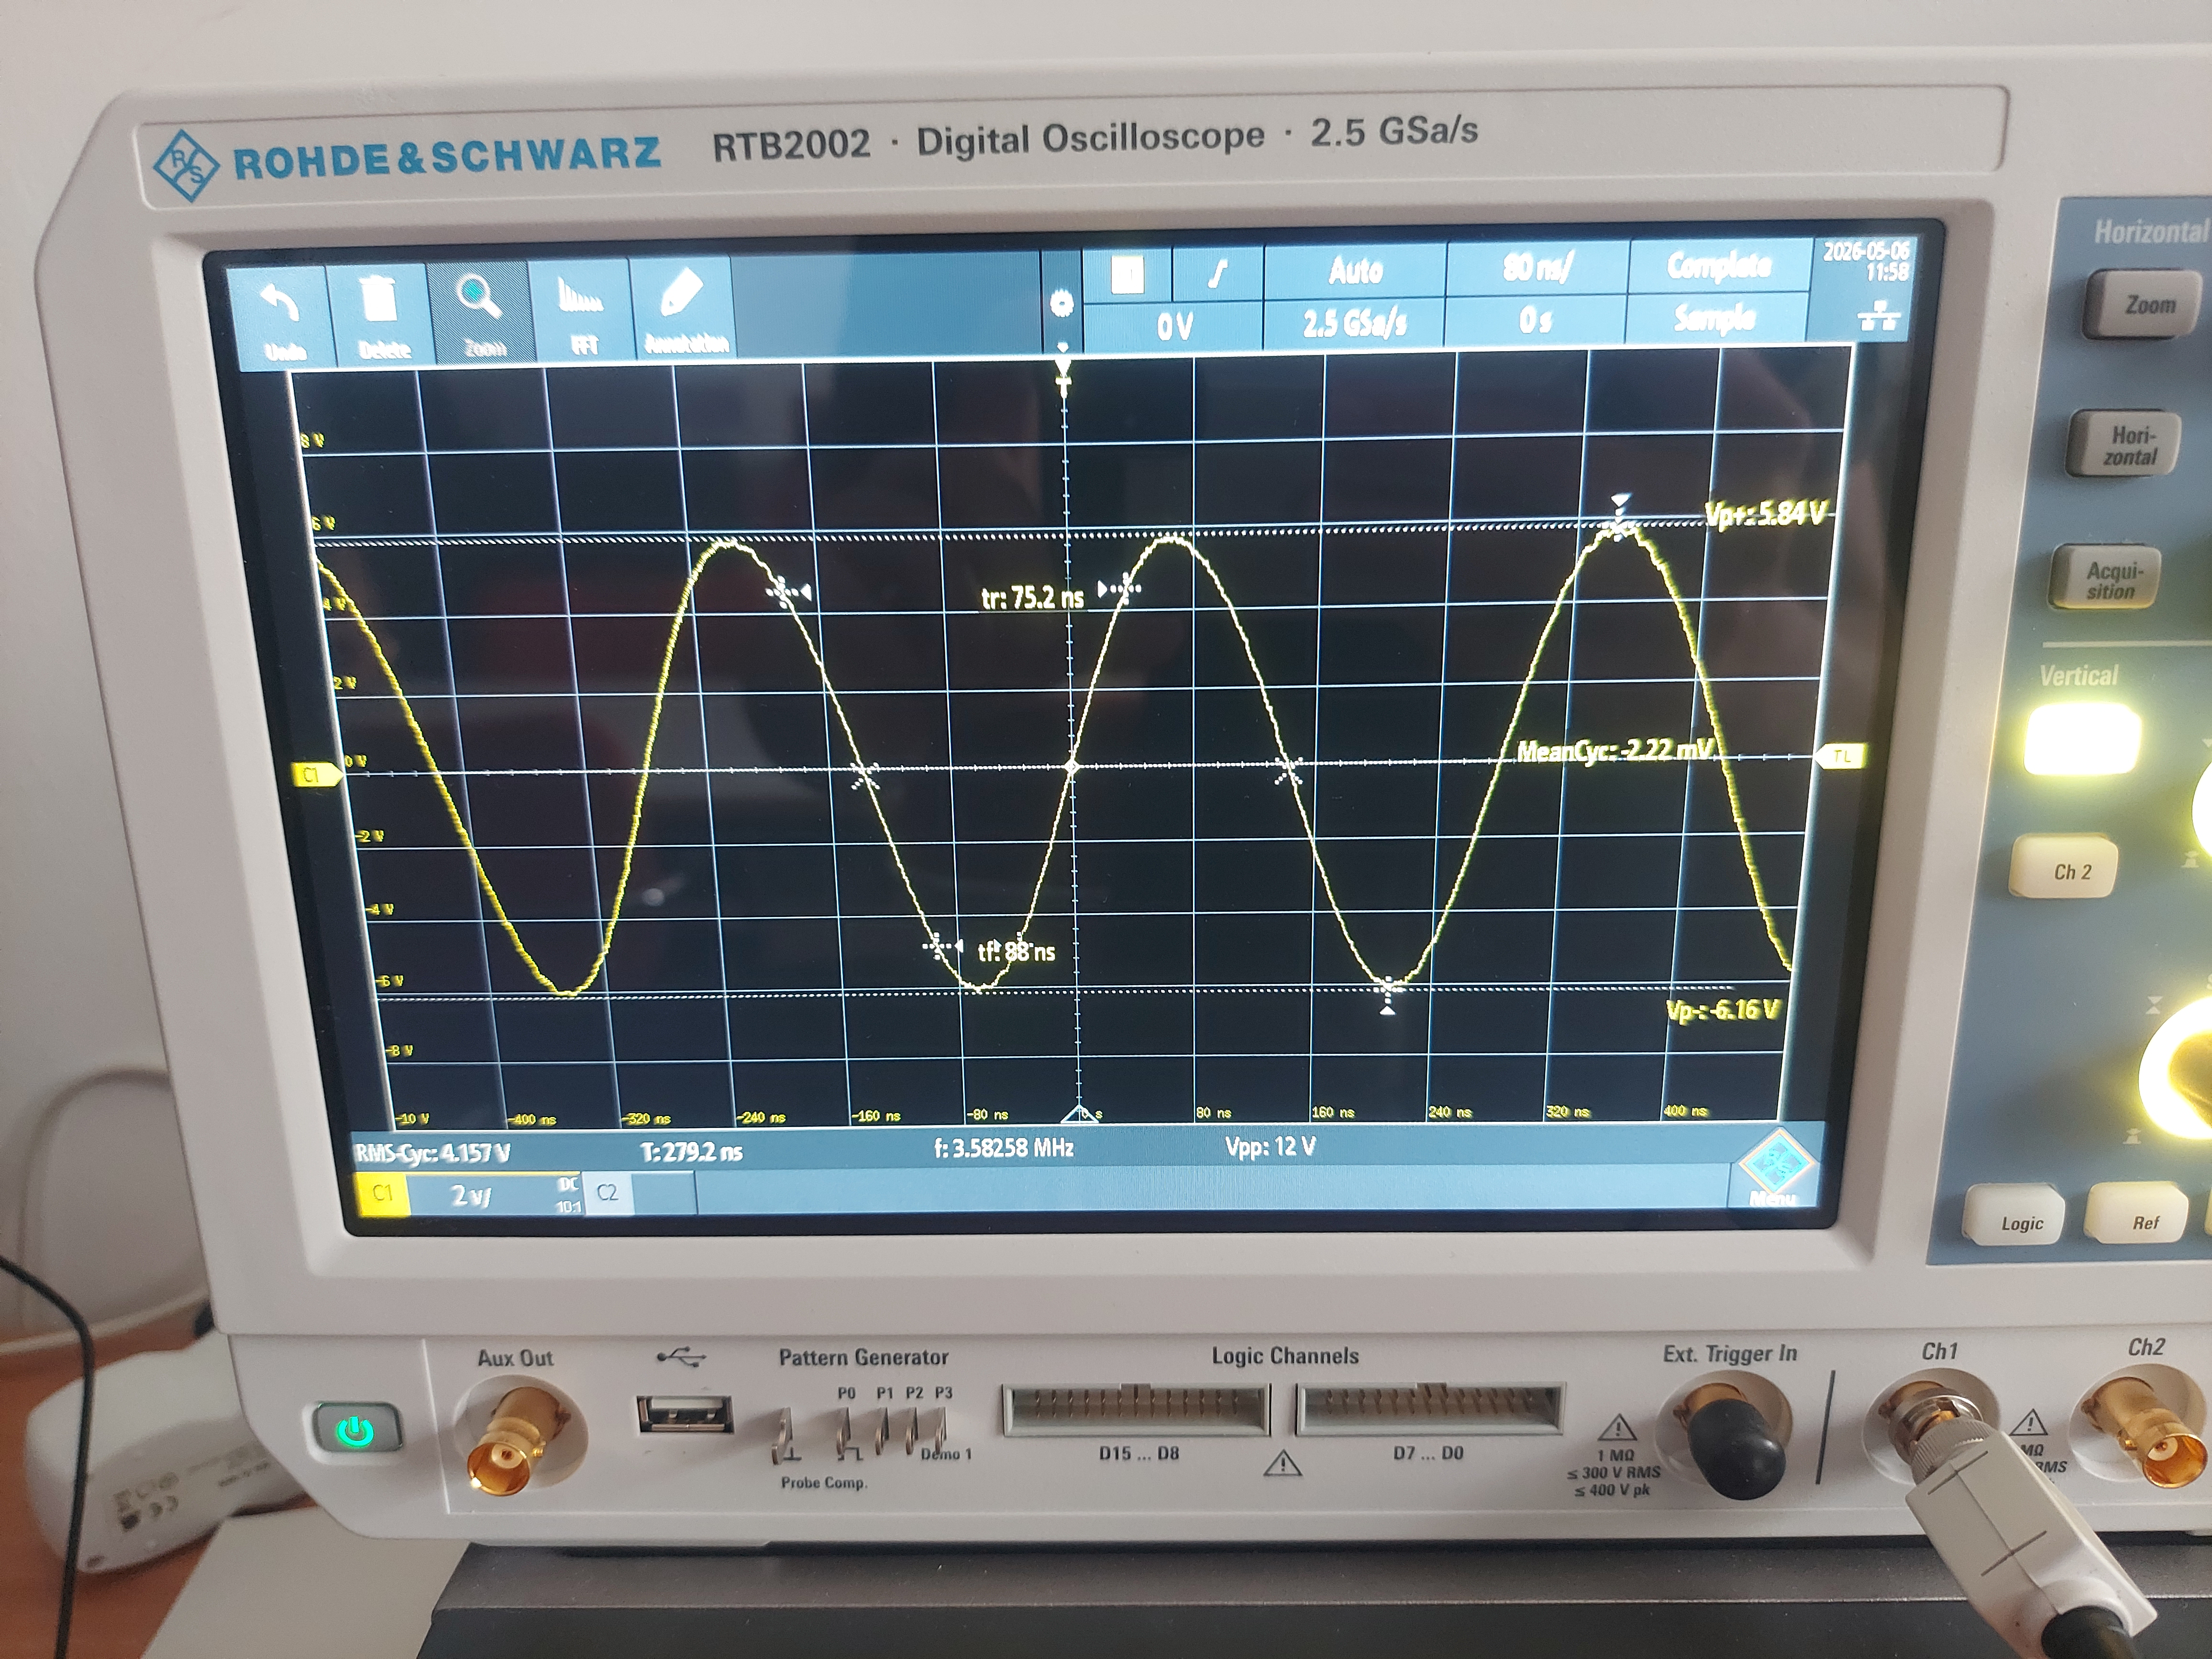
\includegraphics[width=\textwidth]{7measure_tx.jpg}
    \caption{Adás mérése}
\end{figure}

\end{document}